\documentclass[doktyp=studarbeit]{TUBAFarbeiten}

\usepackage{selinput}% Auswahl der Dateikodierung (ansi,latin1,utf8,...)
\usepackage[T1]{fontenc}% Einstellung Fontencoding
\usepackage{amsmath}
\usepackage[section]{placeins}
%\usepackage{titlesec}
\usepackage{xcolor}
\usepackage{listings}
% \usepackage{hyperref}
\usepackage{csquotes}

\newcommand\tab[1][5mm]{\hspace*{#1}}
\newtheorem{thm}{Theorem}
\newtheorem{lem}[thm]{Lemma}
	\SelectInputMappings{adieresis={ä},germandbls={ß},Euro={€}}

% Packages for images and caption in figures
\usepackage{graphicx}
\graphicspath{ {./img/} }
\usepackage{subcaption}

\definecolor{mGreen}{rgb}{0,0.6,0}
\definecolor{mGray}{rgb}{0.5,0.5,0.5}
\definecolor{mPurple}{rgb}{0.58,0,0.82}
\definecolor{backgroundColour}{rgb}{0.95,0.95,0.92}

\lstdefinestyle{C++}{
    backgroundcolor=\color{backgroundColour},   
    commentstyle=\color{mGreen},
    keywordstyle=\color{magenta},
    numberstyle=\tiny\color{mGray},
    stringstyle=\color{mPurple},
    basicstyle=\footnotesize,
    breakatwhitespace=false,         
    breaklines=true,                 
    captionpos=b,                    
    keepspaces=true,                 
    numbers=left,                    
    numbersep=5pt,                  
    showspaces=false,                
    showstringspaces=false,
    showtabs=false,                  
    tabsize=2,
    language=C++
}

\usepackage[backend=biber,sortlocale=de_DE_phonebook]{biblatex}
\addbibresource{references.bib}

%\usepackage{setspace}% Einstellungen Zeilenabstand
	%\onehalfspacing% Einstellungen Zeilenabstand

\TUBAFFakultaet{Fakultät für Mathematik und Informatik}
\TUBAFInstitut{Institut für Informatik}

\TUBAFTitel[OpenGL Game: Achtung, die Kurve!]{OpenGL Game: Achtung, die Kurve!}
\TUBAFBetreuer{M.Sc. Jonas Treumer}
\TUBAFKorrektor{M.Sc. Ben Lorenz}
\TUBAFAutor[Al Nomer/Valdés]{Simon Al Nomer\newline Hernán Felipe Valdés González}
\TUBAFStudiengang{Bachelor Angewandte Informatik}
\TUBAFMatrikel{64\,082\newline 63\,952}
\TUBAFDatum[2020-10-19]{19. Oktober 2020}

\begin{document}

\maketitle

\TUBAFErklaerungsseite

%%%%%%%%%%%%%%%%%%%%%%%%%%%%%%%%%%%%%%%%%%%%%%%%%%%%%%%%%%%%%%%%%%%%%%%%%%%%%%%%
\addsec{Zusammenfassung}
Implementierung des Spieles ''Achtung, die Kurve'' in C++ mit OpenGL für die 
Lehreveranstaltung ''Multimedia''.

%%%%%%%%%%%%%%%%%%%%%%%%%%%%%%%%%%%%%%%%%%%%%%%%%%%%%%%%%%%%%%%%%%%%%%%%%%%%%%%%


\KOMAoptions{
	listof=totoc	% Abbildungs- und Tabellenverzeichnis im Inhaltsverzeichnis
}

\tableofcontents
\listoffigures
\listoftables

\newpage

\section{Einführung}

Achtung, Die Kurve ist ein Multiplayer-Spiel, welches im Jahr 1995 von 
Filip Oščádal und Kamil Doležal in DOS entwickelt wurde. Im Jahr 2010 wurde 
eine neue Version des Spiels unter dem Namen “Achtung, die Kurve! Flash Remake”
veröffentlicht. Diese Version ist mit Adobe Flash von Geert van den Burg 
entwickelt worden und kann online gespielt werden.

Nachdem das Spiel großen Zuspruch fand, beschloss van den Burg, sich mit 
Robin Brouns zusammenzuschließen und eine Fortsetzung zu entwickeln, welche 
2011 unter den Namen Curve Fever (Originaltitel “Achtung, die Kurve! 2”) 
veröffentlicht wurde und online gespielt werden kann.

In den folgenden Jahren wurden dem Spiel immer weiter neue Features 
hinzugefügt wie zum Beispiel verschiedene Boni, die Möglichkeit, in einem Team 
zu spielen, oder das Bestehen einer Rangliste.

2015 sammelte van den Burg ein Team um sich, um eine neue Version des Spiels in 
HTML5 zu implementieren, welche im September 2016 auf den Markt kam.

\begin{figure}[!htb]
    \centering
    \begin{subfigure}[b]{0.45\textwidth}
		\centering
        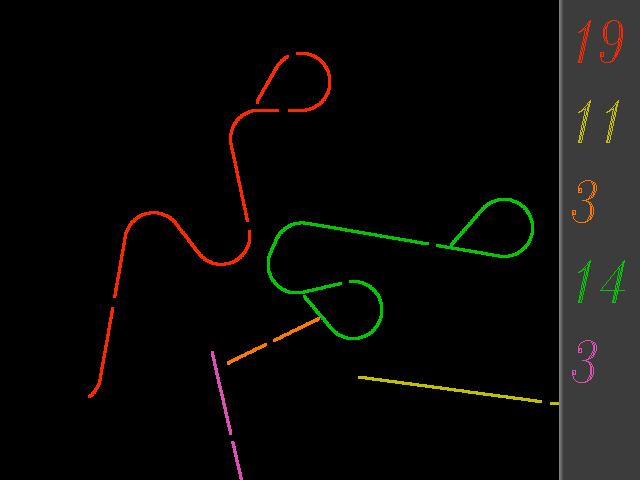
\includegraphics[width=1\linewidth]{dos-version.png}
		\caption{Original version für DOS (1995).}
	\end{subfigure}
	\qquad
	\begin{subfigure}[b]{0.45\textwidth}
		\centering
        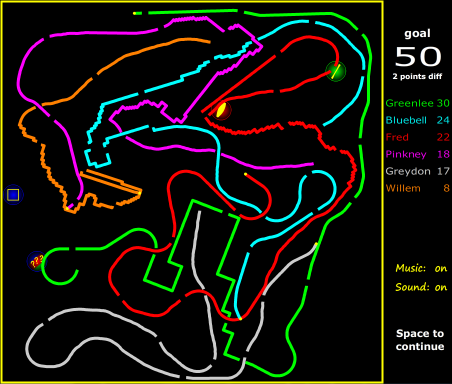
\includegraphics[width=1\linewidth]{flash-version.png}
        \caption{Flash remake (2010).}
	\end{subfigure}
    \caption{2 Versionen, die als Basis für das Spiel genommen wurden.}
	\label{fig:dos-version}
\end{figure}

Die Implementierung unseres Spiels basiert auf die Version von 1995 in 
Kombination mit dem Stil der Flash Version.

\subsection{Spielmechanik}

Im Spiel können bis zu 6 Spieler zusammen mit einem Bildschirm und einer 
Tastatur spielen. Jeder Spieler besitzt zwei vorbestimmten Tasten, die rechts 
und links symbolisieren. Um das Spiel zu starten, müssen mindestens 
2 Spieler spielen.  Der Ziel vom Spiel ist, dass der Spieler am Leben 
solange wie möglich bleibt.

Jeder Spieler wird mit einem Kreis dargestellt, der mit jeder Bewegung einen 
Pfad mit der Farbe des Spielers hinterlässt. Der Spieler darf nur nach rechts 
und links die Richtung seiner Bewegung ändern. Wenn der Spieler nicht reagiert, 
wird er weiter in der alten Richtung sich bewegen.

Ein Spieler verliert, wenn er gegen seine eigene Linie, die Linie anderen 
Spieler,  oder den Rand gestoßen hat. Das Spiel ist zu Ende wenn nur ein 
Spieler noch am Leben ist.

\section{Softwaredokumentation}

Unseres Projekt hat als basis den Code, der zusammen während der Vorlesung 
erstellt wurde, genommen und in C++ migriert. 
Die Entscheidung, um das Spiel in C++ statt C zu programmieren, lag 
insbesondere wegen der Standardbibliothek von C++ und deren implementierten 
Daten Strukturen sowie die Eigenschaft mit Klassen zu programmieren.

Für die Softwarearchitektur wurde das State Pattern implementiert, um einen 
endlichen Automaten zu simulieren und die Änderungen der Zuständen sind in der 
Klasse \textit{Game} durchgeführt.

Das Spiel wurde im Sinne von Szenen programmiert. Die Klasse \textit{Game}
verhaltet sich als eine Szene sowie als eine Szene-Manager. Die anderen
2 Szenen sind \textit{Menu} und \textit{GameOver}.

In dem Spiel wird zwischen User und Player differenziert. Das Spiel besitzt nur
ein User, der die kontrolle über den Computer besitzt und mehrere Players, 
welche die Kreise kontrollieren.

\subsection{user\_data\_t}

Die Daten von dem laufenden Spiel, sowie die Anzahl an Spieler und ihren Punkten
werden in einem Struct gespeichert, der dann in GLFW zur Verfügung gestellt wird.
Dieser Struct heißt \textit{user\_data\_t}.

\begin{lstlisting}[style=C++]
typedef struct {
    int window_width;
    int window_height;
    GameState game_state;
    std::vector<player_info_t>* player_info;
} user_data_t;
\end{lstlisting}

\subsection{player\_info}
Alle die Players werden am Anfang des Programmes in main.cpp addiert und dann
im Menü werden als aktiv gesetzt.

\begin{lstlisting}[style=C++]
typedef struct {
    bool is_active;
    int id;
    std::string name;
    std::string menu_text;
    Control control;
    std::array<GLubyte, 3> color;
    glm::vec3 menu_color;
    int score;
} player_info_t;
\end{lstlisting}

\subsection{Game}

\begin{figure}
    \centering
    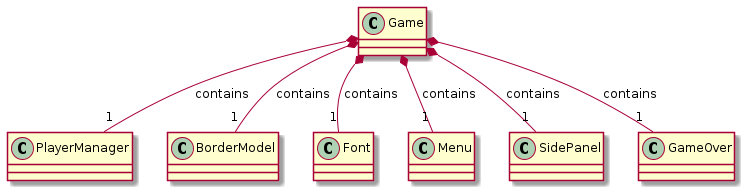
\includegraphics[width=0.9\linewidth]{Game.png}
	\caption{UML Diagramm von der Klasse Game}
	\label{fig:game-uml}
\end{figure}

Die zentrale Klasse unseres Projektes ist \textit{Game}. In dieser Klasse 
werden die Zustände von unseren Automat geändert und unterschiedliche Klassen 
initialisiert und geteilt. In der Abb. \ref{fig:game-uml} steht die 
Klassen, die dann im \textit{Game} initialisiert werden. Ein Beispiel ist die 
Klasse \textit{Font}, die von der Erzeugung und Zeichnung von Text
verantwortlich ist, wird nur einmal in \textit{Game} initialisiert.  

\subsection{GameState}

In der Abb. \ref{fig:state-machine} wird der Automat des Spieles dargestellt. 
Der Startzustand unseres Automaten ist GAME\_MENU. 

\begin{figure}
    \centering
    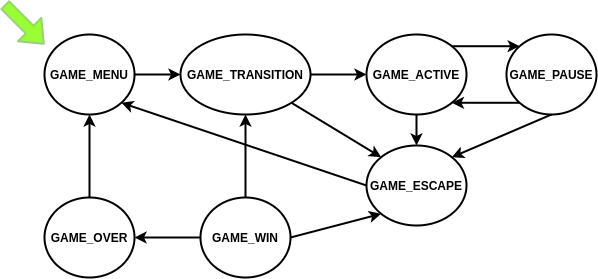
\includegraphics[width=0.7\linewidth]{state_machine.png}
	\caption{Darstellung unseren Zustandsautomat}
	\label{fig:state-machine}
\end{figure}

\paragraph{GAME\_MENU}
Es wird das Menü für den Auswahl von Spieler gezeigt. Man kann nur zu den
nächsten Zustand gehen, GAME\_TRANSITION, in dem man mindestens 2 Spieler
ihre Anwesenheit bestätigen und dann die SPACE-Taste gedrückt wird.
\paragraph{GAME\_TRANSITION}
Das Spiel ist bereit zu starten. Alle Spieler sind in ihren Plätze und ihren
Position wird mit einem gefarbten Kreis gezeichnet. Um das Spiel zu starten
muss die Leertaste gedrückt werden und der neuer Zustand wird GAME\_ACTIVE sein.
Um zurück ins Menü zu gehen, muss die ESCAPE-Taste gedrück werden und der neuer
Zustand wird GAME\_ESCAPE.
\paragraph{GAME\_ACTIVE}
Das Spiel läuft und die Spieler dürfen anderen schließen und in die Irre führen.
Man kann in jedem Moment die SPACE-Taste drücken, um das Spiel zu pausieren,
und der neuer Zustand wird GAME\_PAUSE. Man kann auch mit der ESCAPE-Taste das
Spiel abbrechen und zurück ins Menü gehen, dann der neuer Zustand wird 
GAME\_ESCAPE. Wenn nur ein Spieler übrig auf dem Feld ist, der Zustand wird 
automatisch zu GAME\_WIN oder GAME\_OVER gehen, abhängig ob die maximalle 
Punktzahl erreicht wurde oder nicht.
\paragraph{GAME\_PAUSE}
Das Spiel ist pausiert. Man kann zurück zu GAME\_ACTIVE mit der SPACE-Taste
gehen oder zu GAME\_ESCAPE mit der ESCAPE-Taste.
\paragraph{GAME\_ESCAPE}
Zwischenzustand um die Daten wieder ins Default bringen. Es wird direkt zu 
GAME\_MENU gehen.
\paragraph{GAME\_WIN}
Zwischenzustand um den Gewinner der Runde zu zeigen (mit einem blinken Namen).
Nach ein paar Frames wird direkt zu GAME\_TRANSITION gehen umd eine neue Runde
zu starten. 
\paragraph{GAME\_OVER}
Es wird eine Liste mit der gesamten Punktzahl gezeigt. Wenn man den SPACE-Taste
druck, geht man zu GAME\_MENU und startet alles von vorne.

\subsection{Model und Mesh}
Die Klassen \textit{Model} und \textit{Mesh} sind zwei abstrakte Klassen, welche
als Basis Klasse angewandt werden.

\paragraph{Mesh} 
Ein \textit{Mesh} enthält die Punkte, die gezeichnet werden, das 
Vertex Array Object (VAO) und das Vertex Buffer Object (VBO). 
Die Klassen \textit{BorderMesh}, \textit{PlayerMesh} und \textit{LineMesh} 
erben von \textit{Mesh}, welche die Funktion ''draw'' deklarieren müssen,
um die Punkte zu zeichnen.

\paragraph{Model} 
Ein \textit{Model} enthält ein \textit{Mesh} und die ID von dem \textit{Shader},
das angewandt wird. Ein \textit{Model} interagiert mit \textit{Game} und in
dieser Klasse werden die Positionen und Transformation informiert werden, 
durch die Funktion ''update''.

\subsection{Display}

Die Klasse \textit{Display} initialisiert und besitzt ein Instanz von GLFWwindow. 
Ein Pointer von dem Fenster wird dann mit der Klasse \textit{Game} mitgeteilt. 
\textit{Display} wird dann am Ende des Programms auch das Fenster schließen 
(beenden).

Das Fenster hat ein ursprünglichen Ratio von 1:1 mit der Größe 700x700 pixels.
Das Fenster wird sein Aspect Ratio behalten, in dem immer die kleinste Wert 
zwischen Höhe und Breite nimmt und dann positioniert sich in der Mitte von der 
gegende Position. z.B: Wenn die Höhe größer als die Breite ist, zentriert das 
Fenster sich in der Mitte von der Höhe mit der Größe von der Breite, der Rest
wird ein mit einem schwarzen Padding gefüllt.

\begin{figure}[!htb]
    \centering
    \begin{subfigure}[b]{0.55\textwidth}
        \centering
        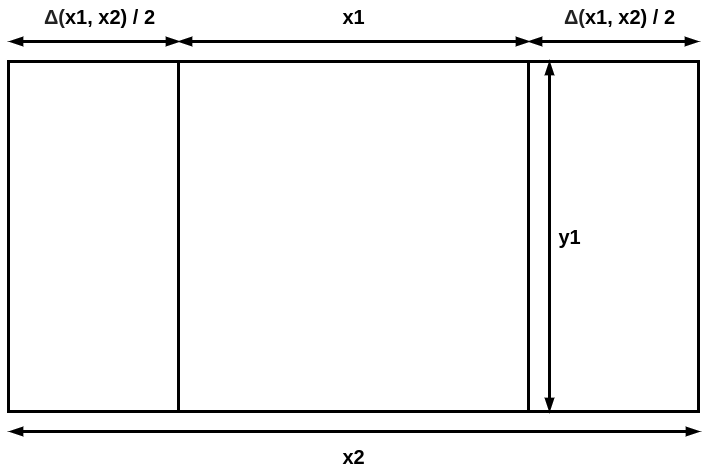
\includegraphics[width=1\linewidth]{display-2.png}
        \caption{Anpassung in horizontellen Resize}
    \end{subfigure}
    \begin{subfigure}[b]{0.4\textwidth}
        \centering
        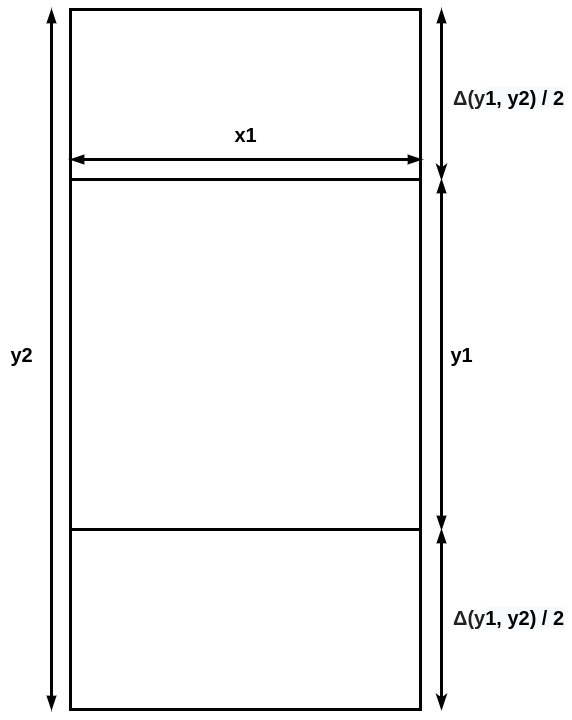
\includegraphics[width=1\linewidth]{display-3.png}
        \caption{Anpassung in vertikallen Resize}
    \end{subfigure}
    \caption{Anpassungen bei der Änderung in der Größe des Fensters}
	\label{fig:display}
\end{figure}

\begin{figure}[!htb]
    \centering
    \begin{subfigure}[b]{0.517\textwidth}
        \centering
        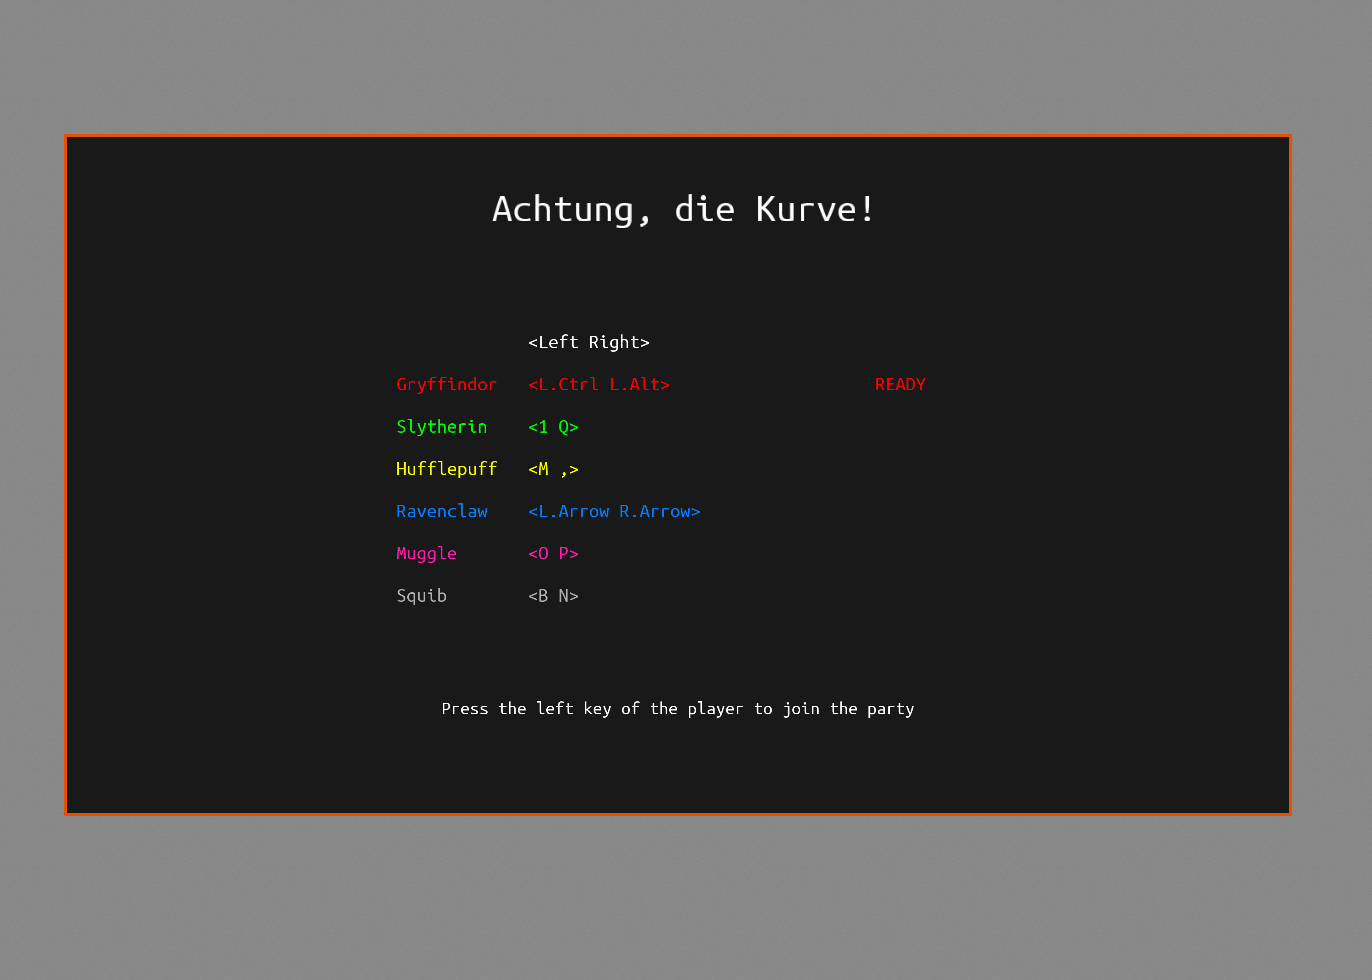
\includegraphics[width=1\linewidth]{aspect-ratio-1.png}
        \caption{Erstellung von den Punkten mit der Kreis-Gleichung}
    \end{subfigure}
    \begin{subfigure}[b]{0.45\textwidth}
        \centering
        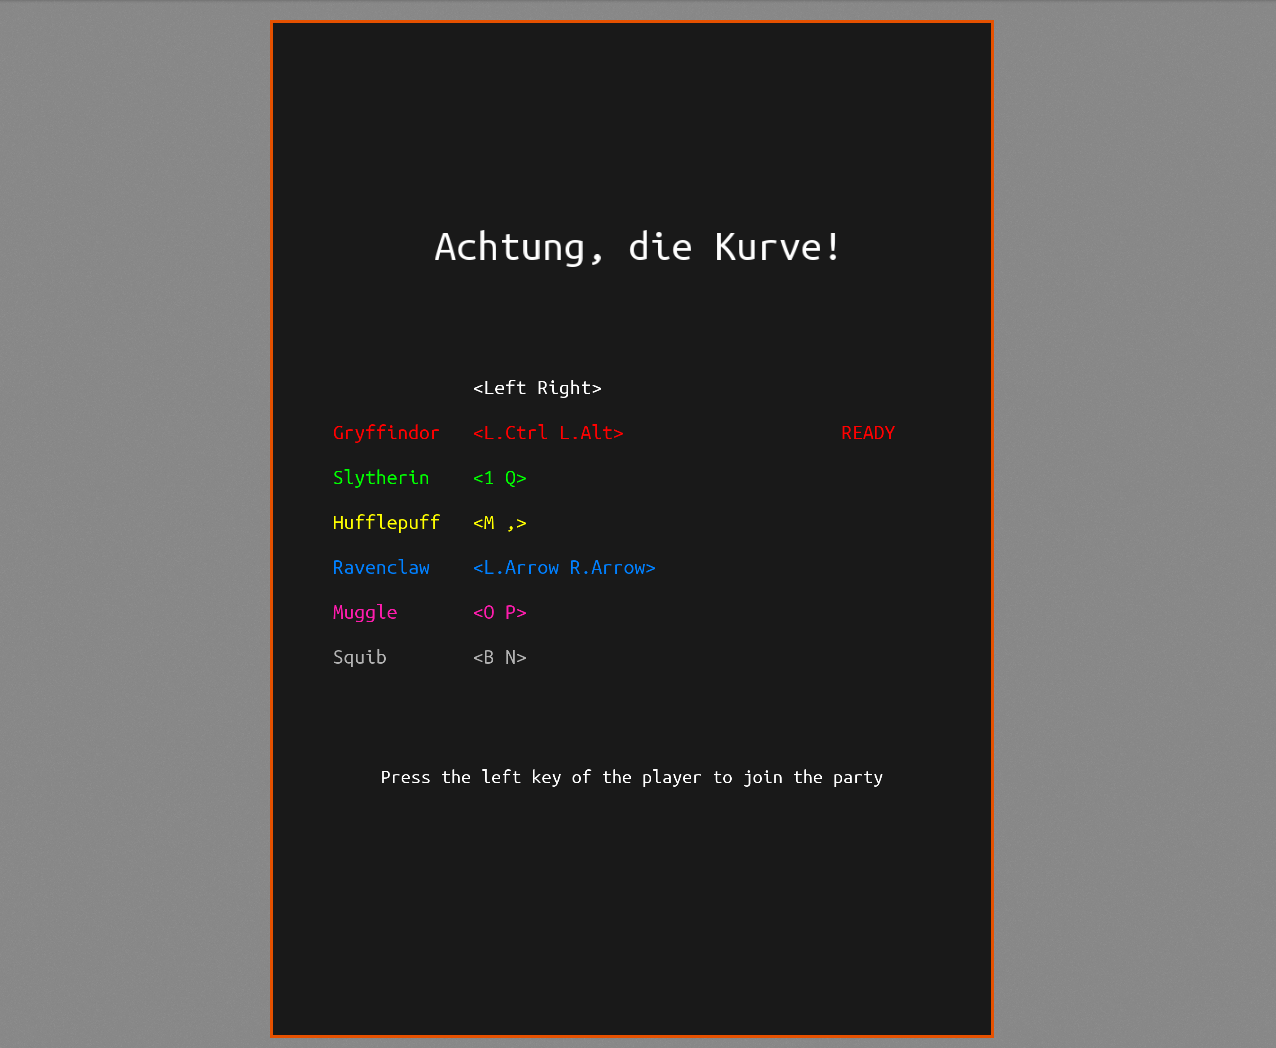
\includegraphics[width=1\linewidth]{aspect-ratio-2.png}
        \caption{Darstellung von GL\_TRIANGLE\_STRIP}
    \end{subfigure}
    \caption{Screenshots von dem Beispiel beim Resizing}
	\label{fig:display-aspect-ratio}
\end{figure}


\section{Zeichnungen}

\subsection{Player}

\begin{figure}[!htb]
    \centering
    \begin{subfigure}[b]{0.4\textwidth}
        \centering
        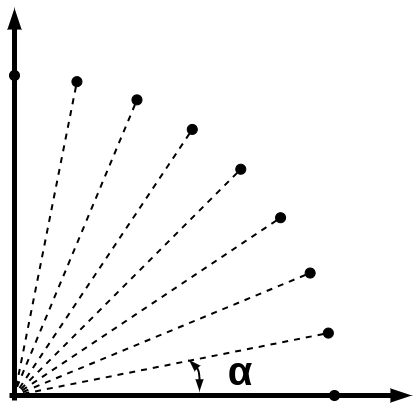
\includegraphics[width=0.8\linewidth]{kreis-1.png}
        \caption{Erstellung von den Punkten mit der Kreis-Gleichung}
    \end{subfigure}
    \begin{subfigure}[b]{0.4\textwidth}
        \centering
        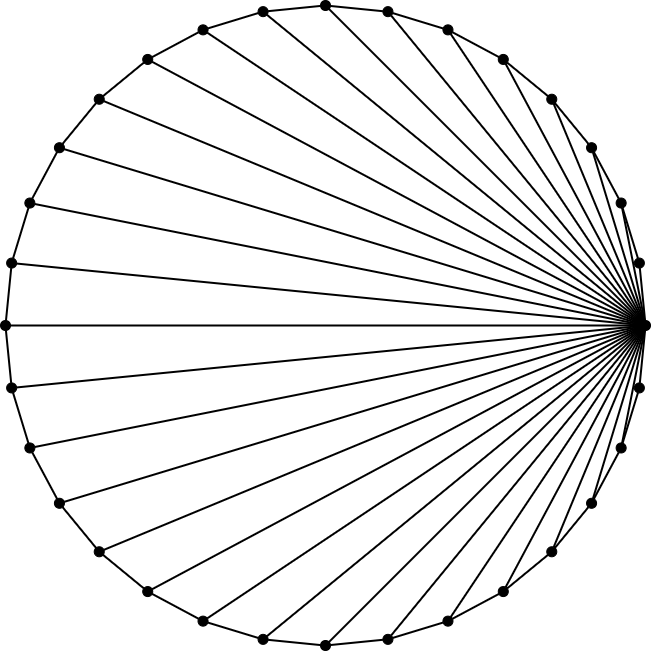
\includegraphics[width=0.8\linewidth]{kreis-2.png}
        \caption{Darstellung von GL\_TRIANGLE\_STRIP}
    \end{subfigure}
    \caption{Darstellung der Erstellung eines Kreises}
    \label{fig:player}
\end{figure}

Jeder Spieler wird mit einem Kreis dargestellt. Die Kreise werden erstellt, in
dem ausgewählte Punkte aus dem Kreis gesammelt werden und sie mit dem 
OpenGL Flag GL\_TRIANGLE\_STRIP zeichnet. Eine Darstellung von dem Prozess
wird in der Abb. \ref{fig:player} gezeigt.

\subsection{Linien}

Für die Zeichnung von dicken Linien wurde ein Algorithmus entwickelt.

Sei $L$ ein Array mit den Punkten in dem der Player befand.
Für die aller erste 2 Punkten in $L$ wird weiter

\begin{figure}[!htb]
    \centering
    \begin{subfigure}[b]{0.45\textwidth}
        \centering
        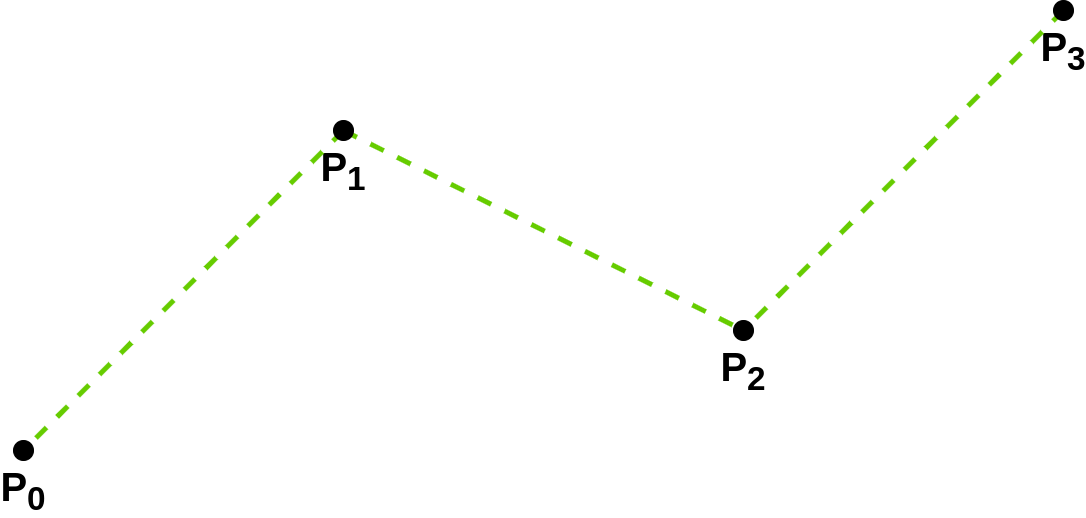
\includegraphics[width=1\linewidth]{Schlangenlinie-1.png}
        \caption{Schritt 1}
    \end{subfigure}
    \qquad
    \begin{subfigure}[b]{0.45\textwidth}
        \centering
        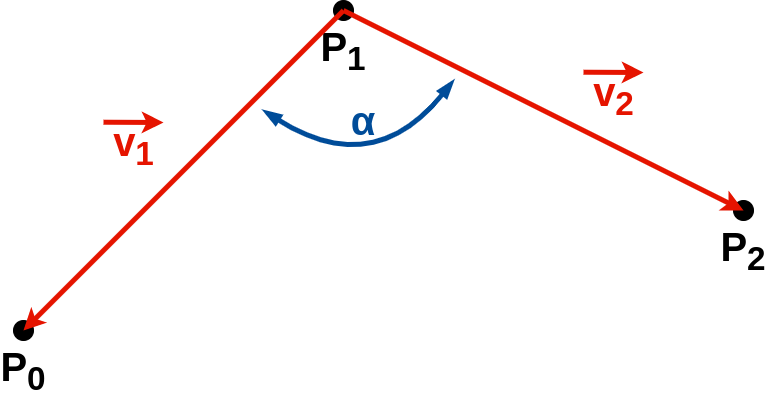
\includegraphics[width=1\linewidth]{Schlangenlinie-2.png}
        \caption{Schritt 2}
    \end{subfigure}
    \qquad
    \begin{subfigure}[b]{0.45\textwidth}
        \centering
        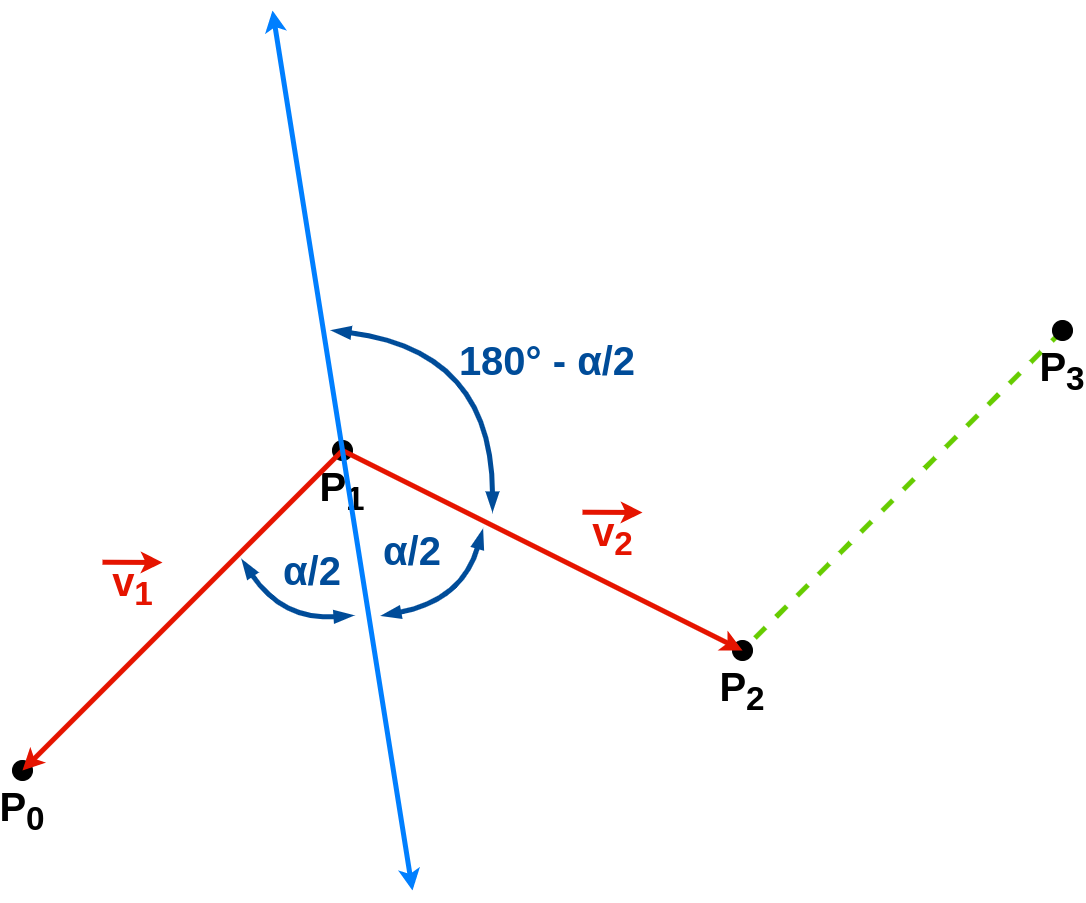
\includegraphics[width=1\linewidth]{Schlangenlinie-3.png}
        \caption{Schritt 3}
    \end{subfigure}
    \qquad
    \begin{subfigure}[b]{0.45\textwidth}
        \centering
        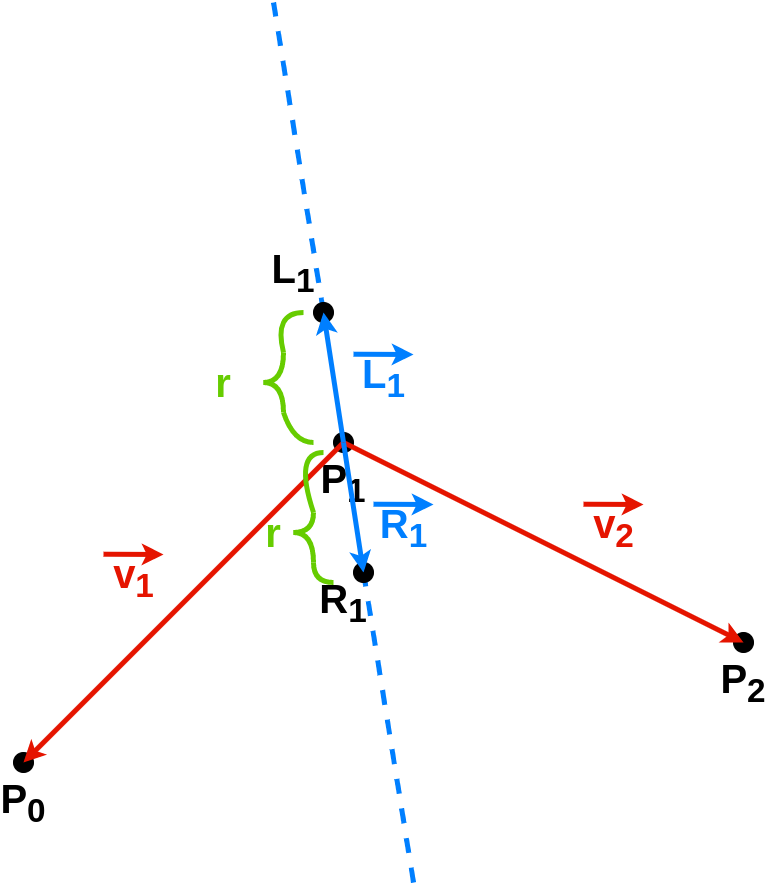
\includegraphics[width=1\linewidth]{Schlangenlinie-4.png}
        \caption{Schritt 4}
    \end{subfigure}
    \qquad
    \begin{subfigure}[b]{0.45\textwidth}
        \centering
        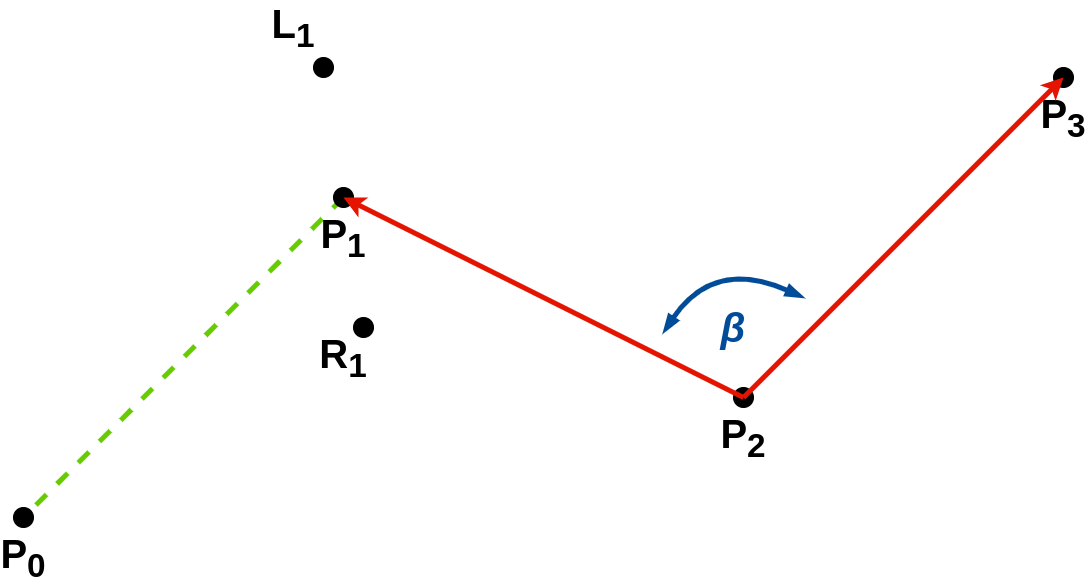
\includegraphics[width=1\linewidth]{Schlangenlinie-5.png}
        \caption{Schritt 5}
    \end{subfigure}
    \qquad
    \begin{subfigure}[b]{0.45\textwidth}
        \centering
        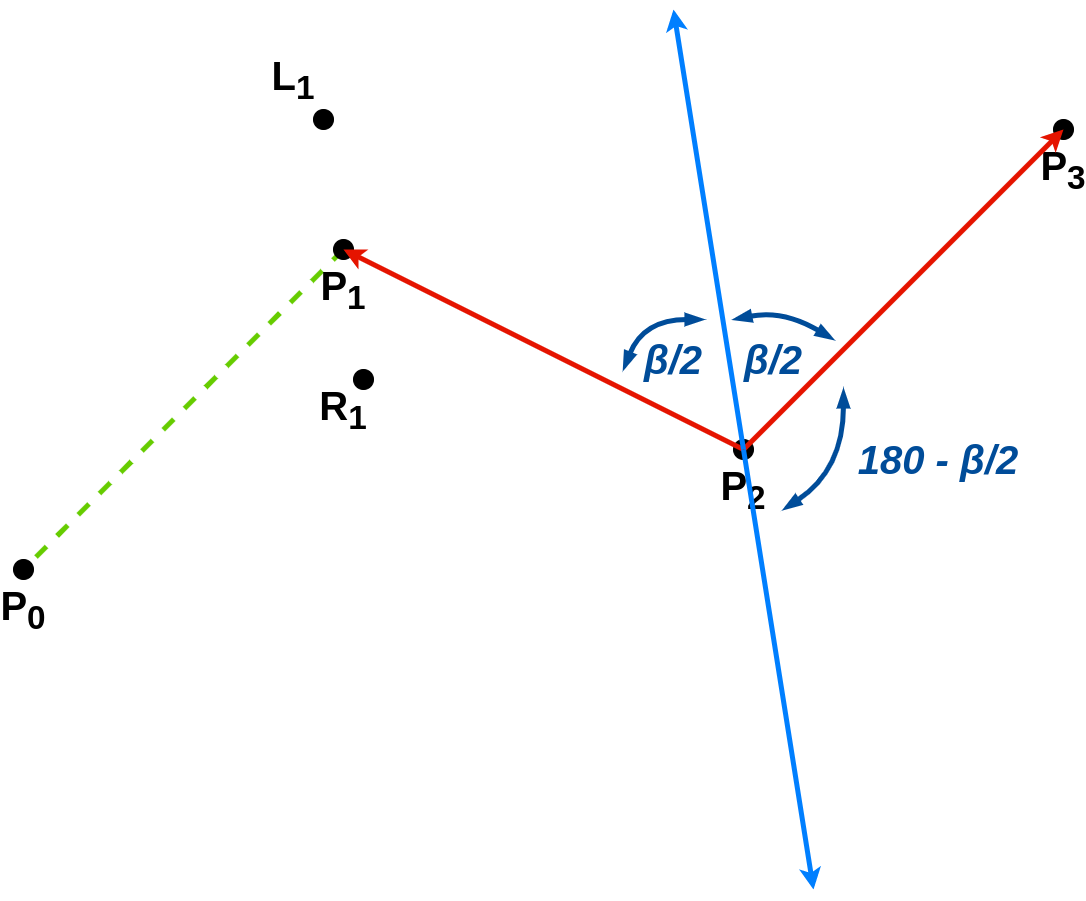
\includegraphics[width=1\linewidth]{Schlangenlinie-6.png}
        \caption{Schritt 6}
    \end{subfigure}
    \qquad
    \begin{subfigure}[b]{0.45\textwidth}
        \centering
        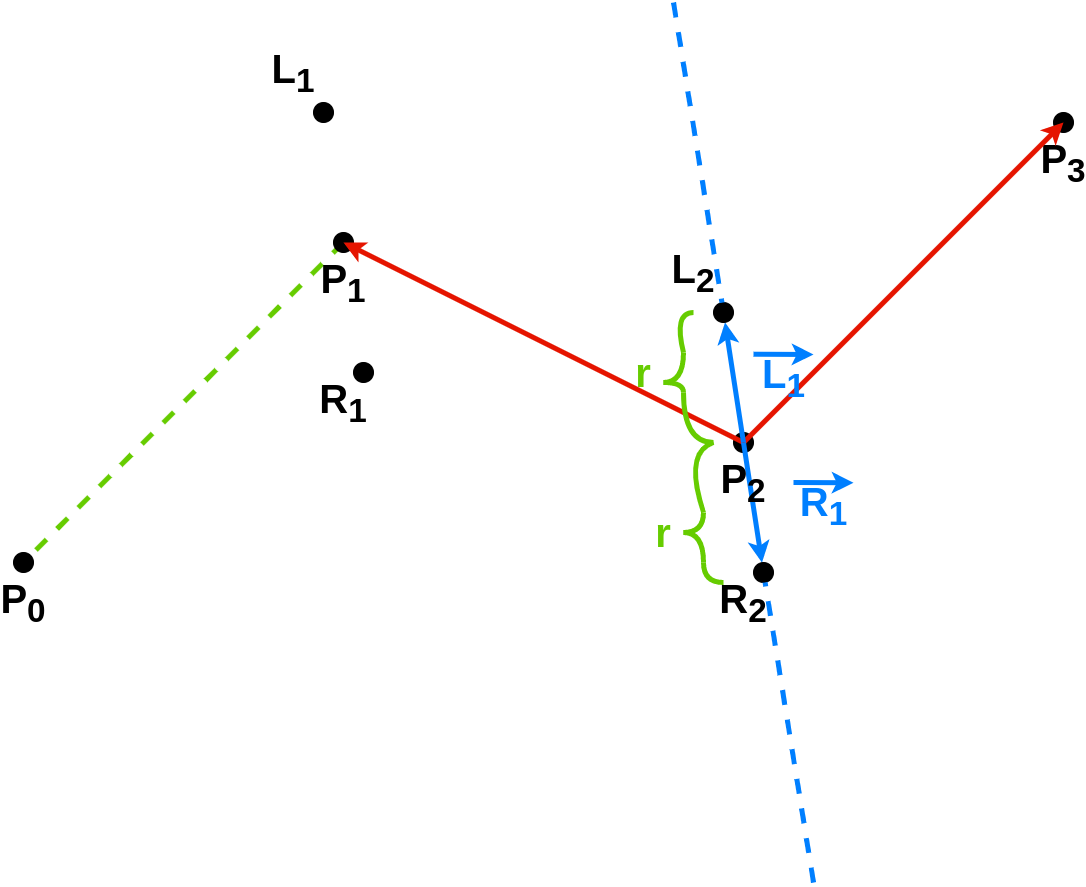
\includegraphics[width=1\linewidth]{Schlangenlinie-7.png}
        \caption{Schritt 7}
    \end{subfigure}
    \qquad
    \begin{subfigure}[b]{0.45\textwidth}
        \centering
        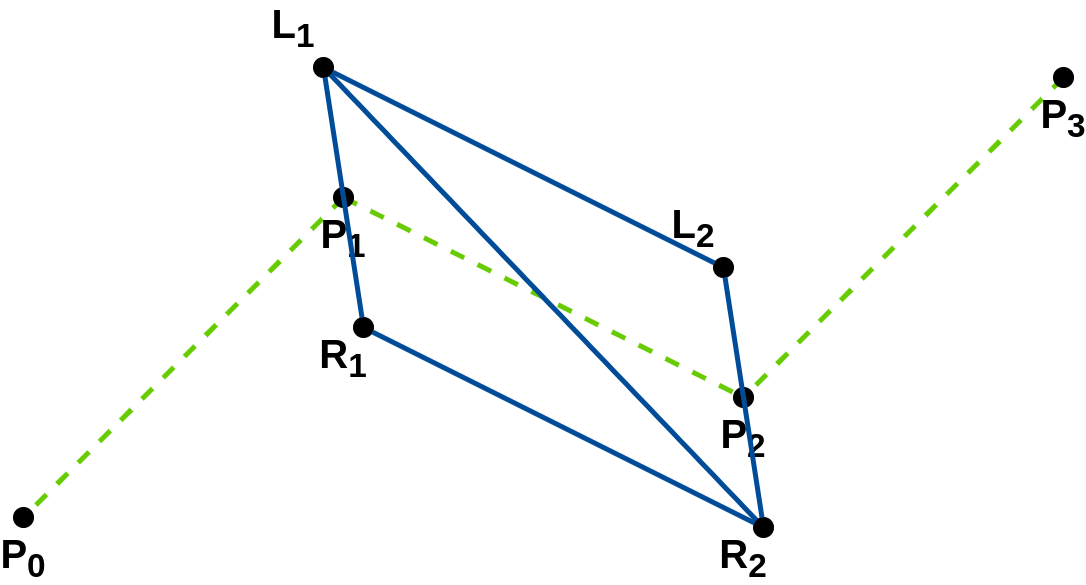
\includegraphics[width=1\linewidth]{Schlangenlinie-8.png}
        \caption{Schritt 8}
    \end{subfigure}
    \caption{Erzeugung eines Linien-Segmenten}
	\label{fig:line}
\end{figure}

\section{Bewegung}

Alle die \textit{PlayerModel}s starten mit einem gleichen 
Geschwindigkeitsvektor $v$.

\begin{equation}
    v =
    \begin{bmatrix}
        0.09    \\
        0
    \end{bmatrix}
\end{equation}

Wenn ein Player initialisiert ist, wird einen randomisierten Winkel $\theta$ 
erzeugt. Dann wird der Vektor $v$ in z rotiert, um einen neuen Vektor zu 
erzeugen.

\begin{equation}
    \begin{bmatrix}
        v'_{x} \\
        v'_{y}     
    \end{bmatrix}
    =
    \begin{bmatrix}
        cos(\theta) & -sin(\theta) \\
        sin(\theta) & cost(\theta)
    \end{bmatrix}
    \begin{bmatrix}
        v_{x} \\
        v_{y}
    \end{bmatrix}
    \label{eq:rotation}
\end{equation}

In jedem Frame gibt es 3 Fälle für alle die aktive Players:

\paragraph{Der Player druck keine Steuerungstaste}
Der Geschwindigkeitsvektor $v$ bleibt gleich und der Player bewegt sich
in die gleiche Richtung.

\paragraph{Der Player druck die linke/rechte Taste}
Der Geschwindigkeitsvektor $v$ wird wie in der Gleichung \ref{eq:rotation}
rotiert.

\paragraph{Der Player ist tot}
Der Player wird nicht mehr geupdated, der Geschwindigkeitsvektor bleibt gleich
aber er wird sich nicht bewegen.

\section{Kollisionen}

Als eine Vereinfachung werden alle Punkte in den Linien als Kreisen betrachtet.

\section{Projektdokumentation}

\section{Benutzerhandbuch}

\begin{figure}[!htb]
	\centering
	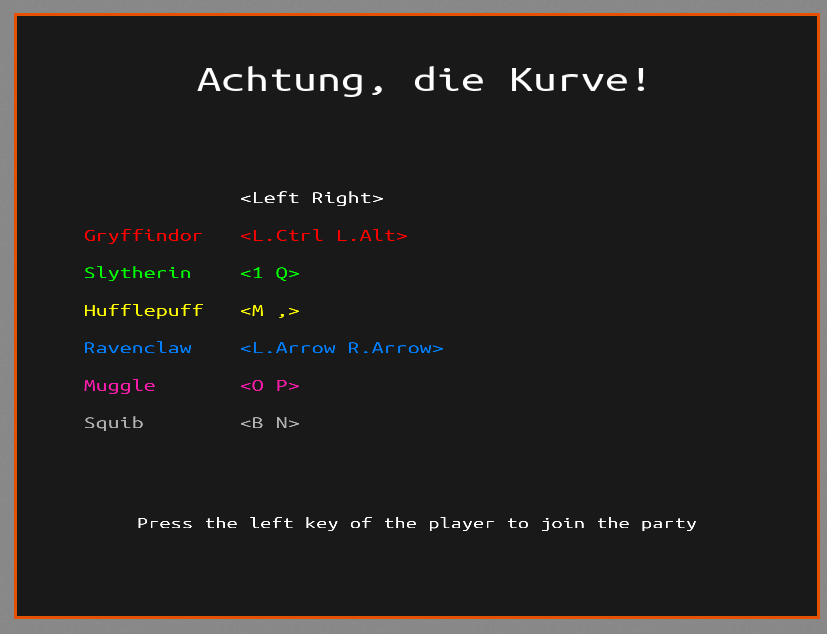
\includegraphics[width=0.8\linewidth]{1.png}
	\caption{Menü Szene.}
	\label{fig:menu}
\end{figure}

\begin{figure}[!htb]
	\centering
	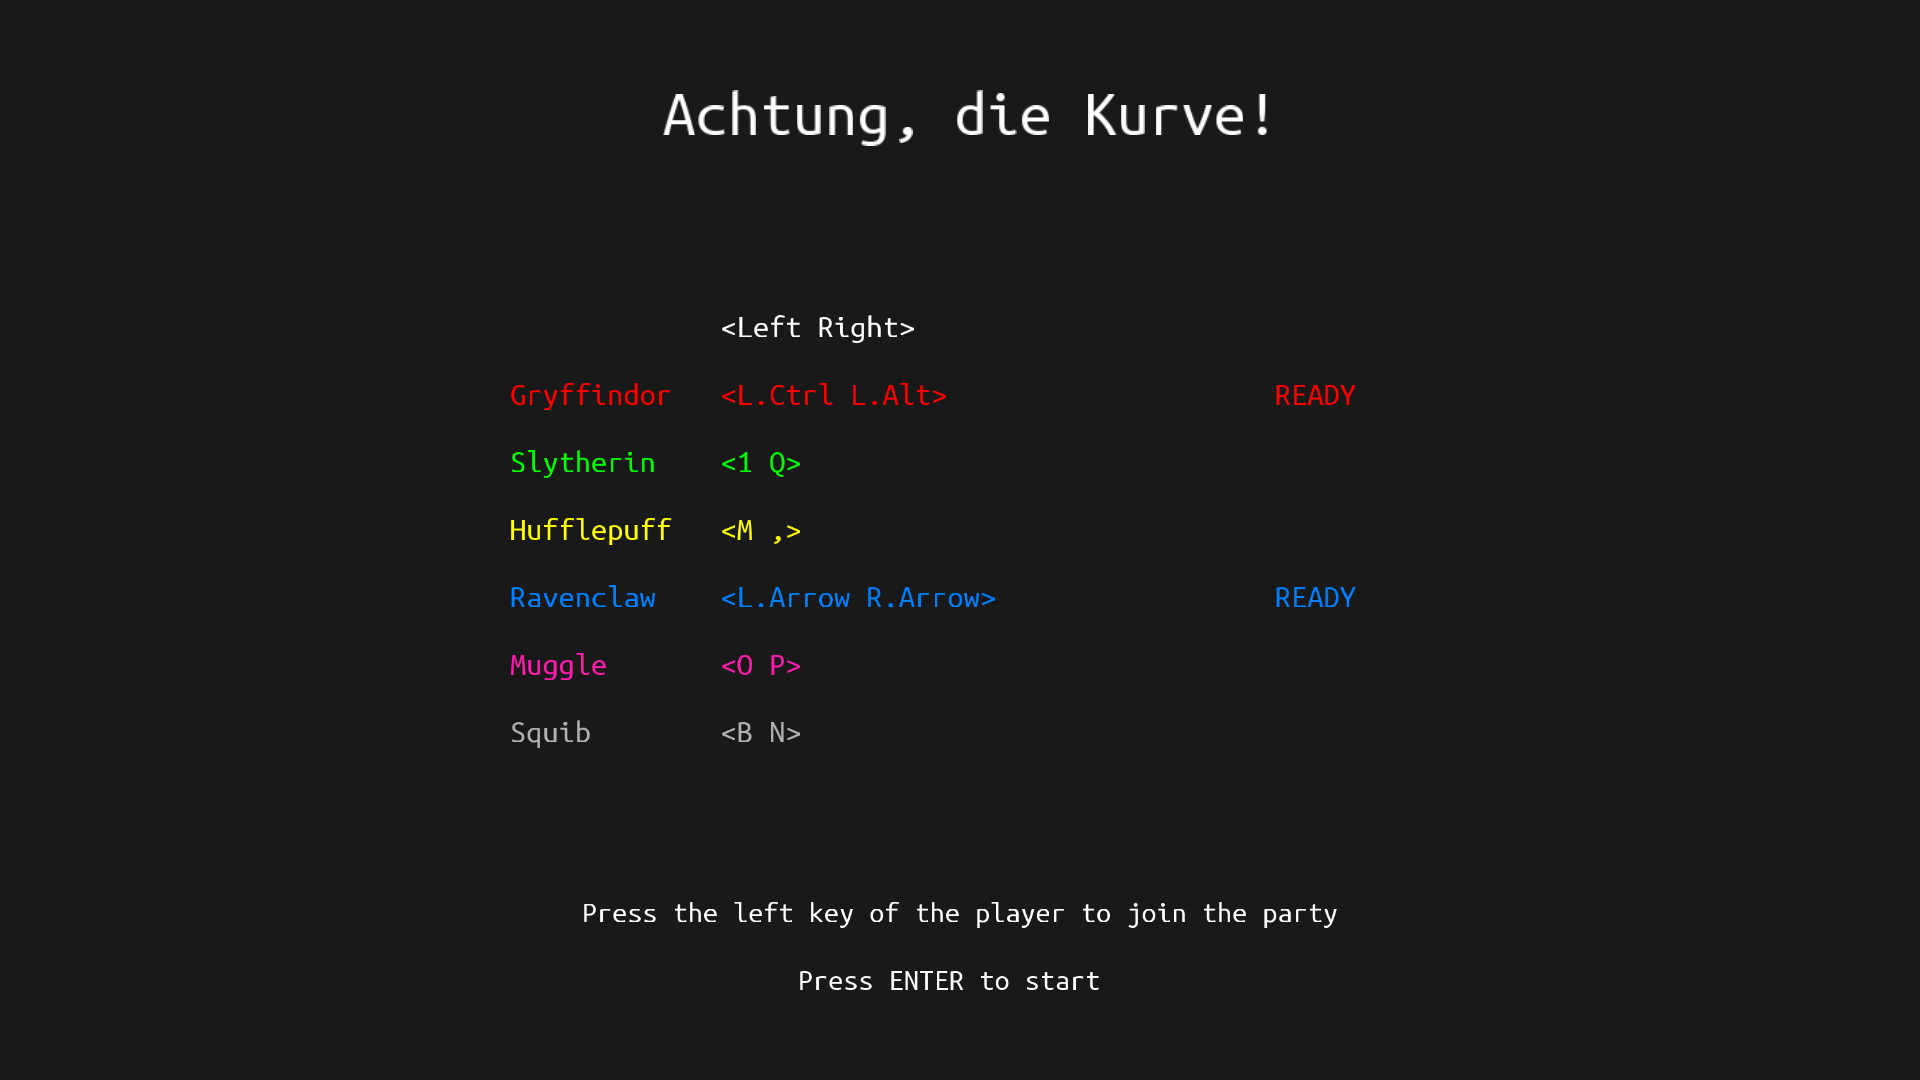
\includegraphics[width=0.8\linewidth]{2.png}
	\caption{Bestätigung der Anwesenheit von Spieler.}
	\label{fig:confirmation}
\end{figure}

\begin{figure}[!htb]
	\centering
	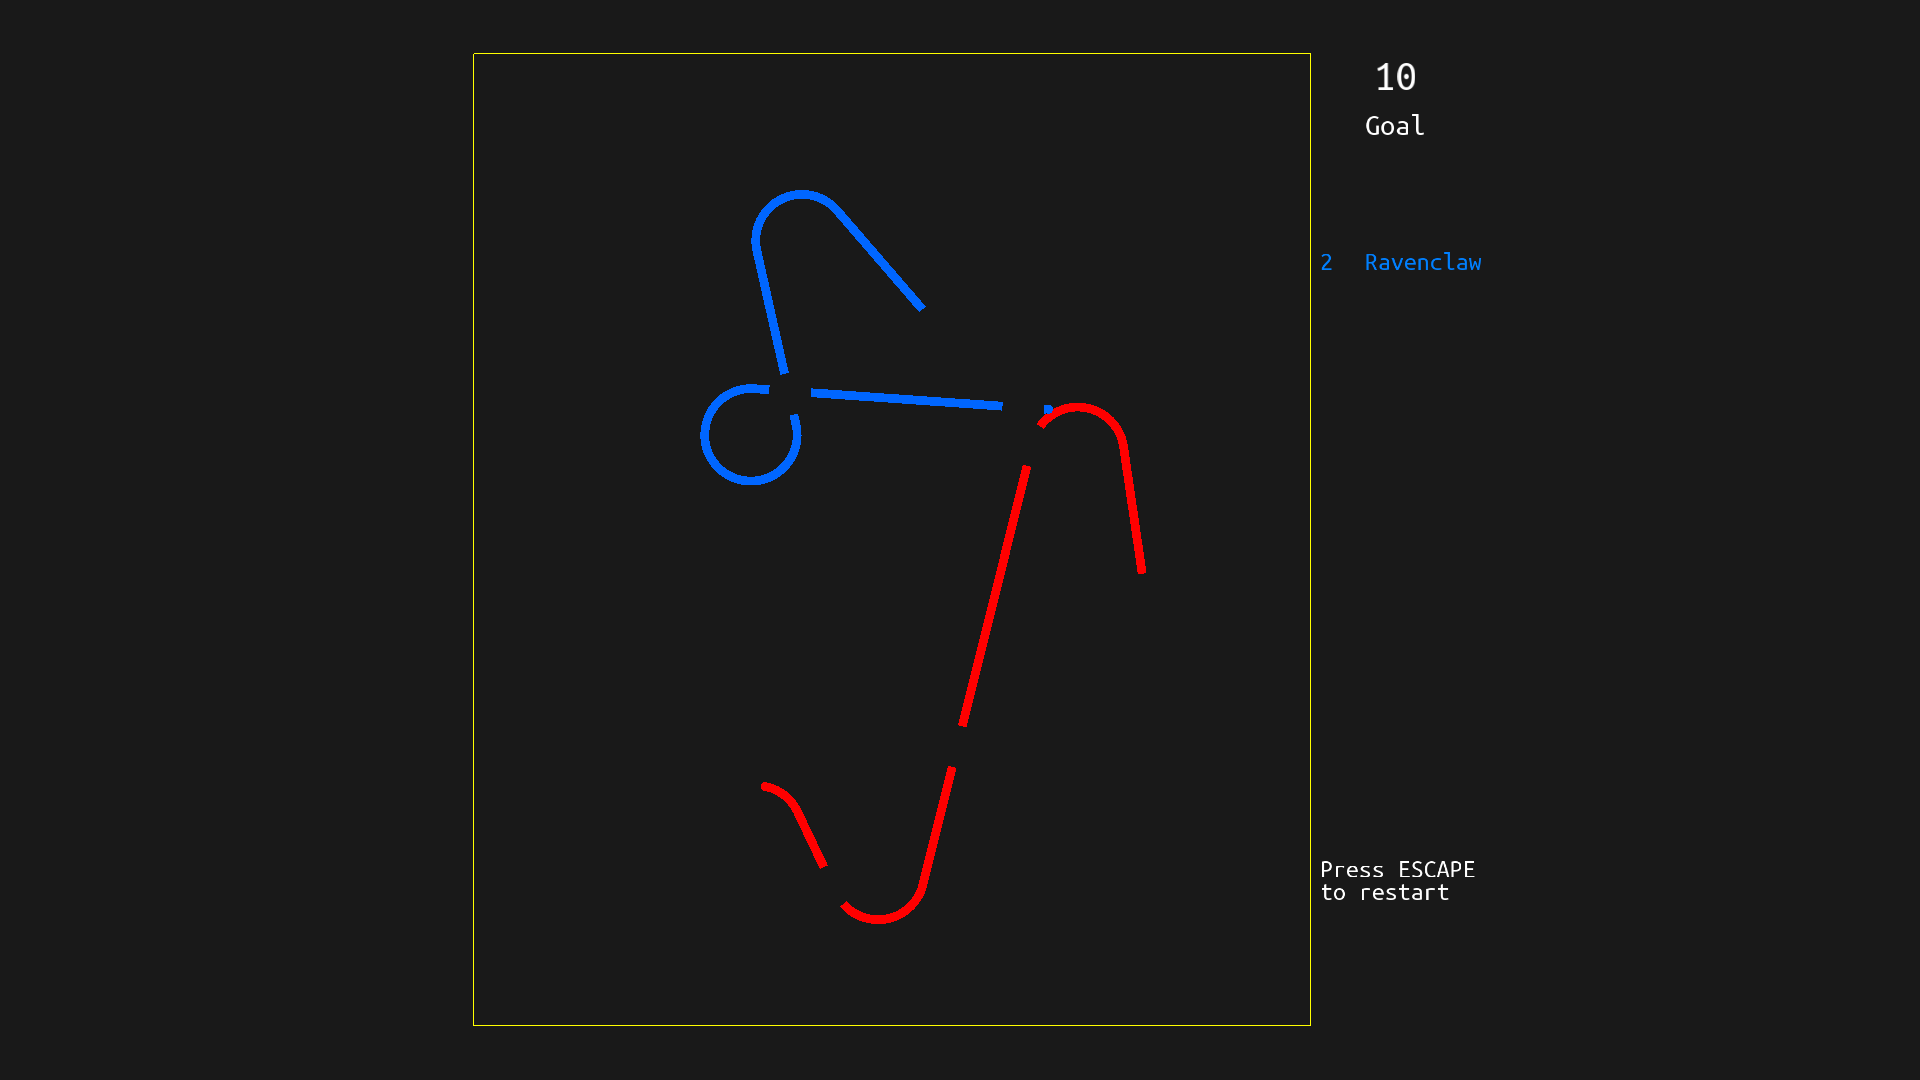
\includegraphics[width=0.8\linewidth]{5.png}
	\caption{Ein Spiel pausiert.}
	\label{fig:pause}
\end{figure}


\printbibliography[heading=bibintoc]

\end{document}